\documentclass[12pt]{article}
\usepackage{graphicx}
\usepackage{cite}
\usepackage{CJK}
\usepackage{amsmath}
\usepackage[colorlinks,linkcolor=black,anchorcolor=blue,citecolor=blue,urlcolor=red]{hyperref}
\usepackage{parskip}
\usepackage{color}
\setlength{\parindent}{0cm}

\begin{document}
\begin{CJK*}{UTF8}{gbsn}
\title{\textbf{Adding toroidal flow in GEM for adiabatic electron model}}
\author{汤炜康}
\date{\today}
\maketitle
\tableofcontents
\newpage

``You don't have to be the chosen one. The secret is to build the resolve and spirit 
to enjoy the plateaus, the times when it doesn't feel like you're improving and you 
question why you're doing this. If you're patient, the plateaus will become springboards.''

{\hfill --- Steve Nash}

\newpage
\section{Guiding center drift due to toroidal flow}
There are three terms needed to be added in the drift velocity of the guiding center $V_{G}$, 
according to Eq. 21 in \cite{sugama98}, i. e.  

\begin{equation}
    \frac{cm_a}{e_aB}\hat{b} \times (\mathbf{U} \cdot \nabla \mathbf{U}), \label{eq1}
\end{equation}
\begin{equation}
    \frac{cm_av_{\parallel}^{'}}{e_aB} \hat{b} \times (\hat{b} \cdot \nabla \mathbf{U}), \label{eq2}
\end{equation}
\begin{equation}
    \frac{cm_av_{\parallel}^{'}}{e_aB} \hat{b} \times (\mathbf{U} \cdot\nabla\hat{b}). \label{eq3}
\end{equation}

In the right-handed coordinate system (R,Z,$\zeta$), considering the toroidal flow with the form of $\mathbf{U}(\mathbf{R}) = -\omega_0(\psi_p)R^2 \nabla \zeta$,
\begin{equation}
    \mathbf{U} \cdot \nabla \mathbf{U} = - \frac{U^2}{R} \hat{R}
\end{equation}
\begin{equation}
    \begin{split}
        \hat{b} \times (\mathbf{U} \cdot \nabla \mathbf{U}) &= \frac{U^2}{R} \hat{R} \times \hat{b}\\
        &= \frac{U^2}{RB} \hat{R} \times (\frac{f}{R}\hat{\zeta} + \frac{\psi_{p}^{'}(r)}{R}(\frac{\partial r}{\partial R}\hat{Z} - \frac{\partial r}{\partial Z}\hat{R}))\\
        &= \frac{U^2}{RB} (-\frac{f}{R}\hat{Z} + \frac{\psi_{p}^{'}(r)}{R} \frac{\partial r}{\partial R}\hat{\zeta}) \label{eq5}
    \end{split}
\end{equation}

Then Eq. \ref{eq1} becomes  
\begin{equation}
    \frac{cm_aU^2}{e_aB^2R^2}(-f\hat{Z} + \psi_{p}^{'}(r)\frac{\partial r}{\partial R} \hat{\zeta}).
\end{equation}

Eq. 6 $\cdot \nabla x$ is
\begin{equation}
    \frac{cm_aU^2}{e_aB^2R^2} \cdot (-f) \frac{\partial r}{\partial Z}.
\end{equation}

To implement this term, a new variable ${\tt ut}$ needed to be declared, representing the equilibrium toroidal flow. 
Actually, we only need to declare a new variable ${\tt omg}$, then \texttt{ut=-omg*radius}, see \hyperref[app]{\bf Appendix}.

For Eq. 6 $\cdot \nabla y$, 
\begin{equation}
    y = \frac{r_0}{q_0}\int_{0}^{\theta}\hat{q}(r,\theta^{'})d\theta^{'}-\zeta)=\frac{r_0}{q_0}(q\theta_f-\zeta)
\end{equation}
\begin{equation}
    \nabla y = \frac{\partial y}{\partial r} \nabla r + \frac{r_0}{q_0} \hat{q} \nabla \theta - \frac{r_0}{q_0} \nabla \zeta,\label{eqdely}
\end{equation}
where $\hat{q} = q \frac{\partial \theta_f}{\partial \theta}$. 
\begin{equation}
\begin{split}
    \textrm{Eq.}\ 6 \cdot \nabla y &= \frac{cm_aU^2}{e_aB^2R^2}(-f\hat{Z} + \psi_p^{'}(r)\frac{\partial r}{\partial R} \hat{\zeta}) \cdot \nabla y \\
                                   &= \frac{cm_aU^2}{e_aB^2R^2}(-f \frac{\partial y}{\partial r} \frac{\partial r}{\partial Z} - \frac{r_0}{q_0} \hat{q} f 
                                      \frac{\partial \theta}{\partial Z} - \frac{r_0}{q_0R} \psi_p^{'}(r)\frac{\partial r}{\partial R}), 
\end{split}
\end{equation}
{\color{blue}
\begin{equation*}
    \frac{cm_aU^2}{e_aB^2R^2}(-f\hat{Z}\cdot\nabla y + \psi_p^{'}(r)\frac{\partial r}{\partial R} \hat{\zeta}\cdot\nabla y)  
\end{equation*}
}

So far, all the terms about Eq. \ref{eq1} is finished. Let's start with Eqs. \ref{eq2} and \ref{eq3}.
Still in the $(R,Z,\zeta)$ coordinate, one could find Eq. \ref{eq2} is identical to Eq. \ref{eq3} as
\begin{equation}
    \mathbf{U}\cdot\nabla\hat{b} = \hat{b}\cdot\nabla\mathbf{U} = - \frac{Uf}{R^2B}\hat{R} - \frac{U}{R^2B}\psi_p^{'}(r)\frac{\partial r}{\partial Z}\hat{\zeta}.
\end{equation}
To derive Eq. 2 or Eq. 3, 
\begin{equation}
\begin{split}
    &\ \ \ \  \frac{cm_av_{\parallel}^{'}}{e_aB} \hat{b} \times (\mathbf{U}\cdot\nabla\hat{b}) \\&= \frac{cm_av_{\parallel}^{'}}{e_aB}
    [-\frac{Uf^2}{B^2R^3}\hat{Z} + \frac{Uf\psi^{'}_p(r)}{B^2R^3}\frac{\partial r}{\partial R}\hat{\zeta}\\
     &\ \ \ \ -\frac{U}{B^2R^3}\psi_p^{'2}(r)\frac{\partial r}{\partial R}\frac{\partial r}{\partial Z}\hat{R}
     -\frac{U}{B^2R^3}\psi_p^{'2}(r)(\frac{\partial r}{\partial Z})^2\hat{Z}]\\
    &=\frac{cm_av_{\parallel}{'}U}{e_aB^3R^3}[-\psi_p^{'2}(r)\frac{\partial r}{\partial R}\frac{\partial r}{\partial Z}\hat{R}
     -(f^2 + \psi_p^{'2}(r)(\frac{\partial r}{\partial Z})^2)\hat{Z} + f\psi_p^{'}(r)\frac{\partial r}{\partial R}\hat{\zeta}].\label{eq14}
\end{split}
\end{equation}
Then, 
\begin{equation}
\begin{split}
    \textrm{Eq.}\ \ref{eq14} \cdot\nabla x &= -\frac{cm_av_{\parallel}{'}U}{e_aB^3R^3}[\psi_p^{'2}(r)(\frac{\partial r}{\partial R})^2\frac{\partial r}{\partial Z}
    +(f^2 + \psi_p^{'2}(r)(\frac{\partial r}{\partial Z})^2)\frac{\partial r}{\partial Z}]\\
    &= -\frac{cm_av_{\parallel}{'}U}{e_aB^3R^3}[\psi_p^{'2}(r)(\frac{\partial r}{\partial R})^2
       +f^2 + \psi_p^{'2}(r)(\frac{\partial r}{\partial Z})^2]\frac{\partial r}{\partial Z}.
\end{split}
\end{equation}

Using Eq. \ref{eqdely},
\begin{equation}
\begin{split}
    \textrm{Eq.}\ \ref{eq14} \cdot\nabla y =& -\frac{cm_av_{\parallel}{'}U}{e_aB^3R^3}[\psi_p^{'2}(r)\frac{\partial r}{\partial R}\frac{\partial r}{\partial Z}
    (\frac{\partial y}{\partial r}\frac{\partial r}{\partial R} + \frac{r_0}{q_0}\hat{q}\frac{\partial \theta}{\partial R})\\
    &+ (f^2 + \psi_p^{'2}(r)(\frac{\partial r}{\partial Z})^2)(\frac{\partial y}{\partial r}\frac{\partial r}{\partial Z} + 
    \frac{r_0}{q_0}\hat{q}\frac{\partial \theta}{\partial Z})\\
    &+ \frac{r_0}{q_0R}f\psi_p^{'}(r)\frac{\partial r}{\partial R}].
\end{split}
\end{equation}
{\color{blue}
\begin{equation*}
    \begin{split}
        \frac{cm_av_{\parallel}{'}U}{e_aB^3R^3}\bigg[&-\psi_p^{'2}(r)\frac{\partial r}{\partial R}\frac{\partial r}{\partial Z}
        \hat{R}\cdot\nabla y\\
        &- \bigg(f^2 + \psi_p^{'2}(r)(\frac{\partial r}{\partial Z})^2\bigg)\hat{Z}\cdot\nabla y\\
        &+ f\psi_p^{'}(r)\frac{\partial r}{\partial R}\hat{\zeta}\cdot\nabla y\qquad\qquad\quad\bigg]
    \end{split}
\end{equation*}
}

\newpage
\section{Parallel acceleration due to toroidal flow}
An auxiliary guiding center variable $v_{\parallel}{''}$ is defined according to 
\begin{equation}
    \varepsilon = \mu\mathbf{B_\mathrm{0}(R)} + \frac{1}{2}mv_{\parallel}^{''2} - \frac{1}{2}mU^2\mathbf{(R)} + q\Phi_1\mathbf{(R)}
\end{equation}
Notice that $v_{\parallel}{''}$ depends on ($\mathbf{R},\varepsilon,\mu$) but not $\gamma$, and $v_{\parallel}{''}=v_{\parallel}{'}+\mathcal{O}(\delta)$.
The new parallel velocity is defined with $\varepsilon^{\mu}$. Since $d\varepsilon^{\mu}/dt=\mathcal{O}(\delta^2)$,
\begin{equation}
\begin{split}
    mv_{\parallel}''\frac{dv_{\parallel}''}{dt} &= -\mu\frac{dB\mathbf{(R)}}{dt} + m\frac{dU^2}{dt} - q\frac{d\Phi_1}{dt}\\
    &=-\mu v_{\parallel}''\mathbf{b}\cdot\nabla B + mv_{\parallel}''\mathbf{b}\cdot\nabla U^2 - qv_{\parallel}''
    \mathbf{b}\cdot\nabla\Phi_1 + \mathcal{O}(\delta^2)
\end{split}
\end{equation}
We will neglect the $\mathcal{O}(\delta^2)$ terms, which include the parallel nonlinearity.
\begin{equation}
    \frac{dv_{\parallel}''}{dt} = -\frac{\mu}{m}\mathbf{b}\cdot\nabla B + \mathbf{b}\cdot\nabla U^2 - \frac{q}{m}\mathbf{b}\cdot\nabla\Phi_1 + \mathcal{O}(\delta^2)
\end{equation}
Term 1 of the r.h.s. of the above equation is the mirror force, which has been implemented in GEM.

For any scalar $s(r,\theta,\zeta)$,
\begin{equation}
    \mathbf{b}\cdot\nabla s=\frac{1}{B}\frac{\psi_p'}{R}\frac{\partial s}{\partial \theta}\hat{\zeta}\cdot\nabla r \times \nabla\theta
    + \frac{f}{BR^2}\frac{\partial s}{\partial \zeta}.
\end{equation}
{\color{cyan}
\begin{equation*}
\begin{split}
    \mathbf{b}\cdot\nabla s&=\frac{1}{B}(\nabla\zeta\times\nabla\psi_p+\frac{f}{R}\hat{\zeta})\cdot(\frac{\partial s}{\partial r}\nabla r
    +\frac{\partial s}{\partial \theta}\nabla \theta+\frac{\partial s}{\partial \zeta}\nabla \zeta)\\
    &=\frac{\psi_p'}{B}(\nabla\zeta\times\nabla r)\cdot(\frac{\partial s}{\partial r}\nabla r
    +\frac{\partial s}{\partial \theta}\nabla \theta+\frac{\partial s}{\partial \zeta}\nabla \zeta)+\frac{f}{BR^2}\frac{\partial s}{\partial\zeta}\\
    &=\frac{1}{B}\frac{\psi_p'}{R}\frac{\partial s}{\partial \theta}\hat{\zeta}\cdot\nabla r \times \nabla\theta
    + \frac{f}{BR^2}\frac{\partial s}{\partial \zeta}
\end{split}
\end{equation*}
}

So,
\begin{equation}
    \mathbf{b}\cdot\nabla B=\frac{1}{B}\frac{\psi_p'}{R}\frac{\partial B}{\partial \theta}\hat{\zeta}\cdot\nabla r \times \nabla\theta
\end{equation}
\begin{equation}
    \mathbf{b}\cdot\nabla U^2=\frac{2U}{B}\frac{\psi_p'}{R}\frac{\partial U}{\partial \theta}\hat{\zeta}\cdot\nabla r \times \nabla\theta,
\end{equation}
\begin{equation}
    \mathbf{b}\cdot\nabla \Phi_1=\frac{1}{B}\frac{\psi_p'}{R}\frac{\partial \Phi_1}{\partial \theta}\hat{\zeta}\cdot\nabla r \times \nabla\theta
\end{equation}
with
\begin{equation}
    \hat{\zeta}\cdot\nabla r \times \nabla\theta = |\nabla r \times \nabla\theta|.
\end{equation}
The $\partial U/\partial\theta$ and $\partial \Phi_1/\partial\theta$ will be calculated in the \texttt{gem\_equil.f90}. Others are all existing variables in GEM. 
$\Phi_1$ is the electric potential determined by the charge-neutrality, with $\mathbf{E_n}=-\nabla\Phi_1$. For a plasma with a single ion species with ion 
temperature $T_i$ and electron temperature $T_e$, 
\begin{equation}
    e\Phi_1=\frac{m_i\omega_0^2}{2(1+T_i/T_e)}(R^2 - \langle R^2\rangle).
\end{equation}
Attention, here the bracket $\langle\cdots\rangle$ stands for the flux surface average.
\begin{equation}
    \langle R^2\rangle = \frac{1}{2\pi}\int_{-\pi}^{\pi}R^2(r,\theta)d\theta
\end{equation}
Thus,
\begin{equation}
    \partial_{\theta}(R^2 - \langle R^2\rangle) = 2R\partial_{\theta}R-\frac{R^2}{2\pi}
\end{equation}

\newpage
\section{Changes in weight equation} 
Let $f=f_0+\delta f$, the perturbed part of distribution function
\begin{equation}
    \delta f = -q(\phi - \mathbf{U\cdot A})\frac{f_0}{T} + h
\end{equation}
Here, $h$ is the non-adiabatic part of $\delta f$. 

Write $h=h + h_1 + h_2 \cdots$
\begin{equation}
    h_2 = \delta f + \frac{q}{T}f_0 [(\phi - \mathbf{U\cdot A}) - \langle(\phi - \mathbf{U\cdot A})\rangle + \langle\mathbf{v'\cdot A}\rangle]
\end{equation}
\begin{equation}
\begin{split}
    \ \ \ \ &\frac{\partial h_2}{\partial t} + \langle\mathbf{\dot{R}}\rangle\cdot\nabla h_2 + \langle\dot{\varepsilon}^u\rangle\frac{\partial h_1}{\partial\varepsilon^u}
    - \langle\dot{\varepsilon}^u\rangle\frac{\partial }{\partial\varepsilon^u}\langle\frac{q}{T}f_0\mathbf{v'\cdot A}\rangle\\
    =&-\bigg\langle\frac{d\mathbf{R}}{dt}\bigg|_1\bigg\rangle\cdot\frac{\partial f_0}{\partial\mathbf{R}}\\
    &-q\mathbf{v}_g\cdot\nabla\langle\Psi\rangle\frac{f_0}{T}\\
    &+q[\mathbf{U(R)}\cdot\nabla\langle\Psi\rangle-\langle\mathbf{U}\cdot\nabla\Psi\rangle]\frac{f_0}{T}\\
    &-\frac{q}{\Omega}\bigg\langle(\nabla\Psi\times\mathbf{b})\cdot\nabla\psi_p\ \omega_0'R\bigg(\frac{B_t}{B_0}v_\parallel'+U\bigg)\bigg\rangle\frac{f_0}{T}\\
    &+S_1+S_2+S_3
\end{split}
\end{equation}
There are two terms to be added in the weight equation. For electrostatic model, $\Psi=\phi$.

The first term, 
\begin{equation}
\begin{split}
    q[\mathbf{U(R)}\cdot\nabla\langle\phi\rangle-\langle\mathbf{U}\cdot\nabla\phi\rangle]\frac{f_0}{T}
\end{split}
\end{equation}
All right, let's proceed a further step. Write
\begin{equation}
    \mathbf{U(x)=U(R) + \boldsymbol{\rho}\cdot\nabla U},
\end{equation}
then
\begin{equation}
    \begin{split}
        \mathbf{U(R)}\cdot\nabla\langle\phi\rangle-\langle\mathbf{U}\cdot\nabla\phi\rangle=-\langle\boldsymbol{\rho}\cdot\nabla \mathbf{U}\cdot\nabla\phi\rangle.
    \end{split}
\end{equation}
{\color{cyan}Remember,
\begin{equation*}
\hat{\zeta}\cdot\nabla\hat{R}=\frac{1}{R}\hat{\zeta}\ \textrm{and}\ \hat{\zeta}\cdot\nabla\hat{\zeta}=-\frac{1}{R}\hat{R}.   
\end{equation*}
These two terms results from the reconverting from the Cartesian coordinate to the cylindrical coordinate in deriving the material derivative,
see Eq. 7.106 in \cite{vc}.

\begin{equation*}
    \boldsymbol{\rho} = \rho(\mathbf{e_1}\textrm{sin}\gamma + \mathbf{e_2}\textrm{cos}\gamma),
\end{equation*}
where $\rho = v_{\perp}'/\Omega=\sqrt{2\mu B/m}/(qB/m), \mathbf{e_1}=\nabla r/|\nabla r|, \mathbf{e_2}=\mathbf{b}\times\mathbf{e_1}$ and 
$\gamma$ is the gyro angle.

Let
\begin{equation*}
    \bf{e_1}=\rm{e_{1R}}\it(r,\theta)\hat{R} + \rm{e_{1Z}}\it(r,\theta)\hat{Z}
\end{equation*}
\begin{equation*}
    \bf{e_2}=\rm{e_{2R}}\it(r,\theta)\hat{R} + \rm{e_{2Z}}\it(r,\theta)\hat{Z} + \rm{e_{2\zeta}}\it(r,\theta)\hat{\zeta},
\end{equation*} 
then we have
\begin{equation*}
    \boldsymbol{\rho}=\rho\bigg(({\rm e_{1R}sin}\gamma + {\rm e_{2R}cos}\gamma)\hat{R}
    + ({\rm e_{1Z}sin}\gamma + {\rm e_{2Z}cos}\gamma)\hat{Z} + ({\rm e_{2\zeta}cos}\gamma)\hat{\zeta}\bigg)
\end{equation*}
}
\begin{equation}
    \begin{split}
        \boldsymbol{\rho}\cdot\nabla \mathbf{U}&=\boldsymbol{\rho}\cdot\nabla(U\hat{\zeta})\\
        &=\boldsymbol{\rho}\cdot\nabla U\hat{\zeta} + U\boldsymbol{\rho}\cdot\nabla \hat{\zeta}\\
        &=\boldsymbol{\rho}\cdot\bigg(\frac{U}{R}\hat{R}-\omega'R\frac{\partial r}{\partial R}\hat{R}-\omega'R\frac{\partial r}{\partial Z}\hat{Z}\bigg)\hat{\zeta}
        -\frac{U\rho_\zeta}{R}\hat{R}\\
        &=\bigg(\frac{U\rho_R}{R} -\omega'R\frac{\partial r}{\partial R}\rho_R-\omega'R\frac{\partial r}{\partial Z}\rho_Z\bigg)\hat{\zeta}
        -\frac{U\rho_\zeta}{R}\hat{R}\\
    \end{split}
\end{equation}

\begin{equation}
    \begin{split}
        &\bigg(\frac{U\rho_R}{R} -\omega'R\frac{\partial r}{\partial R}\rho_R-\omega'R\frac{\partial r}{\partial Z}\rho_Z\bigg)\hat{\zeta}\cdot\nabla\phi\\ 
        =&\bigg(\frac{U\rho_R}{R} -\omega'R\frac{\partial r}{\partial R}\rho_R-\omega'R\frac{\partial r}{\partial Z}\rho_Z\bigg)\hat{\zeta}\cdot\frac{\partial\phi}{\partial y}\nabla y\\
        =&\bigg(-\frac{U\rho_R}{R} +\omega'R\frac{\partial r}{\partial R}\rho_R+\omega'R\frac{\partial r}{\partial Z}\rho_Z\bigg)\frac{r_0}{q_0R}\frac{\partial\phi}{\partial y}  
    \end{split}
\end{equation}

\begin{equation}
    \begin{split}
        -\frac{U\rho_\zeta}{R}\hat{R}\cdot\nabla\phi &= -\frac{U\rho_\zeta}{R}\hat{R}\cdot\bigg(\frac{\partial\phi}{\partial x}\nabla x
        + \frac{\partial\phi}{\partial y}\nabla y + \frac{\partial\phi}{\partial z}\nabla z\bigg)\\
        &=-\frac{U\rho_\zeta}{R}\bigg(\frac{\partial\phi}{\partial x}\frac{\partial r}{\partial R} 
        + \frac{\partial\phi}{\partial y}\bigg(\frac{\partial y}{\partial r}\frac{\partial r}{\partial R}
        + \frac{r_0}{q_0}\hat{q}\frac{\partial \theta}{\partial R}\bigg)
        + \frac{\partial \phi}{\partial z}q_0R_0\frac{\partial \theta}{\partial R}\bigg)
    \end{split}
\end{equation}

\begin{equation}
    \begin{split}
        &-\langle\boldsymbol{\rho}\cdot\nabla \mathbf{U}\cdot\nabla\phi\rangle=
        \bigg(\frac{U}{R}\bigg\langle\rho_R\frac{\partial\phi}{\partial y}\bigg\rangle -\omega'R\frac{\partial r}{\partial R}\bigg\langle\rho_R\frac{\partial\phi}{\partial y}\bigg\rangle -\omega'R\frac{\partial r}{\partial Z}\bigg\langle\rho_Z\frac{\partial\phi}{\partial y}\bigg\rangle\bigg)\frac{r_0}{q_0R}\\
        &+\frac{U}{R}\bigg(\bigg\langle\rho_\zeta\frac{\partial\phi}{\partial x}\bigg\rangle\frac{\partial r}{\partial R} 
        + \bigg\langle\rho_\zeta\frac{\partial\phi}{\partial y}\bigg\rangle\bigg(\frac{\partial y}{\partial r}\frac{\partial r}{\partial R}
        + \frac{r_0}{q_0}\hat{q}\frac{\partial \theta}{\partial R}\bigg)
        + \bigg\langle\rho_\zeta\frac{\partial \phi}{\partial z}\bigg\rangle q_0R_0\frac{\partial \theta}{\partial R}\bigg)
    \end{split}
\end{equation}

{\color{blue}
\begin{equation*}
    \begin{split}
        &\bigg[\bigg(\omega'R\frac{\partial r}{\partial R} - \frac{U}{R}\bigg)\bigg\langle\rho_R\frac{\partial\phi}{\partial y}\bigg\rangle + \omega'R\frac{\partial r}{\partial Z}\bigg\langle\rho_Z\frac{\partial\phi}{\partial y}\bigg\rangle\bigg]\hat{\zeta}\cdot\nabla y\\
        +&\frac{U}{R}\bigg(\bigg\langle\rho_\zeta\frac{\partial\phi}{\partial x}\bigg\rangle\frac{\partial r}{\partial R} 
        + \bigg\langle\rho_\zeta\frac{\partial\phi}{\partial y}\bigg\rangle\hat{R}\cdot\nabla y
        + \bigg\langle\rho_\zeta\frac{\partial \phi}{\partial z}\bigg\rangle \hat{R}\cdot\nabla z\bigg)
    \end{split}
\end{equation*}}

\begin{equation*}
    \rho_R = \rho({\rm e_{1R}sin}\gamma + {\rm e_{2R}cos}\gamma)
\end{equation*}
\begin{equation*}
    \rho_Z = \rho({\rm e_{1Z}sin}\gamma + {\rm e_{2Z}cos}\gamma)
\end{equation*}
\begin{equation*}
    \rho_\zeta = \rho{\rm e_{2\zeta}cos}\gamma
\end{equation*}
\begin{equation*}
    {\rm e_{1R}} = \frac{\partial r}{\partial R}\bigg/|\nabla r| = {\tt srbr/gr}
\end{equation*}
\begin{equation*}
    {\rm e_{1Z}} = \frac{\partial r}{\partial Z}\bigg/|\nabla r| = {\tt srbz/gr}
\end{equation*}
\begin{equation*}
    {\rm e_{2R}} = -\frac{f}{RB}{\rm e_{1Z}} 
\end{equation*}
\begin{equation*}
    {\rm e_{2Z}} = \frac{f}{RB}{\rm e_{1R}} 
\end{equation*}
\begin{equation*}
    {\rm e_{2\zeta}} = \frac{\psi_p'}{RB}\bigg[-{\rm e_{1R}}\frac{\partial r}{\partial R} - {\rm e_{1Z}}\frac{\partial r}{\partial Z}\bigg] 
\end{equation*}

The gyro average of $\rho_R, \rho_Z {\rm \ and\ } \rho_\zeta$ could be obtained by the 4-point averaging method.
The 4 points are at $\gamma=\pi/2,3\pi/2,0 {\rm \ and\ }\pi$, respectively.

The second term,
\begin{equation}
\begin{split}
    &-\frac{q}{\Omega}\bigg\langle(\nabla\phi\times\mathbf{b})\cdot\nabla\psi_p\ \omega_0'R\bigg(\frac{B_t}{B_0}v_\parallel'+U\bigg)\bigg\rangle\frac{f_0}{T}\\
    =&-\frac{q}{\Omega}\bigg\langle(\nabla\phi\times\mathbf{b})\cdot\nabla\psi_p\bigg\rangle\omega_0'R\bigg(\frac{B_t}{B_0}v_\parallel'+U\bigg)\frac{f_0}{T}\label{t2}
\end{split}
\end{equation}

Considering
\begin{equation}
\begin{split}
    \mathbf{B}&=\nabla\psi\times\nabla(q\theta_f-\zeta)\\
    &=\frac{q_0}{r_0}\frac{d\psi}{dx}\nabla x\times\nabla y\\
    &=C(x)\nabla x\times\nabla y
\end{split}
\end{equation}
then
\begin{equation}
    \mathbf{b}=\frac{\nabla x\times\nabla y}{|\nabla x\times\nabla y|}.
\end{equation}
So we have
\begin{equation}
    \begin{split}
        \nabla\phi\times\mathbf{b}\cdot\nabla\psi_p &= \nabla\psi_p\times\nabla\phi\cdot\mathbf{b}\\
        &=\psi_p'\nabla x\times\nabla\phi\cdot\frac{\nabla x\times\nabla y}{|\nabla x\times\nabla y|}\\
        &=\frac{\psi_p'}{|\nabla x\times\nabla y|}\bigg(\frac{\partial\phi}{\partial y}\nabla x\times\nabla y
        + \frac{\partial\phi}{\partial z}\nabla x\times\nabla z\bigg)\cdot\nabla x\times\nabla y\\
        &=\psi_p'|\nabla x\times\nabla y|\frac{\partial\phi}{\partial y} {\color{blue}+ \frac{\psi_p'}{|\nabla x\times\nabla y|}
        \frac{\partial\phi}{\partial z}(\nabla x\times\nabla z)\cdot(\nabla x\times\nabla y)}\label{t1}
    \end{split}
\end{equation}
{\color{blue}
\begin{equation}
    \begin{split}
        (\nabla x\times\nabla z)\cdot(\nabla x\times\nabla y)&=(\nabla x\times\nabla y)\times\nabla x\cdot\nabla z\\
        &=(|\nabla x|^2\nabla y - |\nabla x\cdot\nabla y|\nabla x)\cdot\nabla z\\
        &=|\nabla x|^2\nabla y\cdot\nabla z - |\nabla x\cdot\nabla y|\nabla x\cdot\nabla z\\
        &=|\nabla x|^2\nabla y\cdot\nabla z - q_0R_0|\nabla x\cdot\nabla y|\ |\nabla r\cdot\nabla\theta|
    \end{split}
\end{equation}
\begin{equation}
    \begin{split}
        \nabla y\cdot\nabla z &= \bigg(\frac{\partial y}{\partial r}\nabla r + \frac{r_0}{q_0}\hat{q}\nabla\theta 
        - \frac{r_0}{q_0}\nabla\zeta\bigg)\cdot q_0 R_0\nabla\theta\\
        &=q_0R_0\frac{\partial y}{\partial r}|\nabla r\cdot\nabla\theta| + r_0R_0\hat{q}|\nabla\theta|^2\label{t3}
    \end{split}
\end{equation}
}
According to Eq. \ref{t1} - \ref{t3}, Eq. \ref{t2} can be coded using existing variables. The blue parts above are 
small ordering terms that are NOT implemented for now. 

\newpage
\section{Verification of the model}
Above are all the changes for adiabatic electron model. Let's start to test the code. We'll start with the well-known
Cyclone Base Case (CBC), those parameters could be found in Ref. \cite{gorler}. 

\begin{figure}[htb!]
\centering
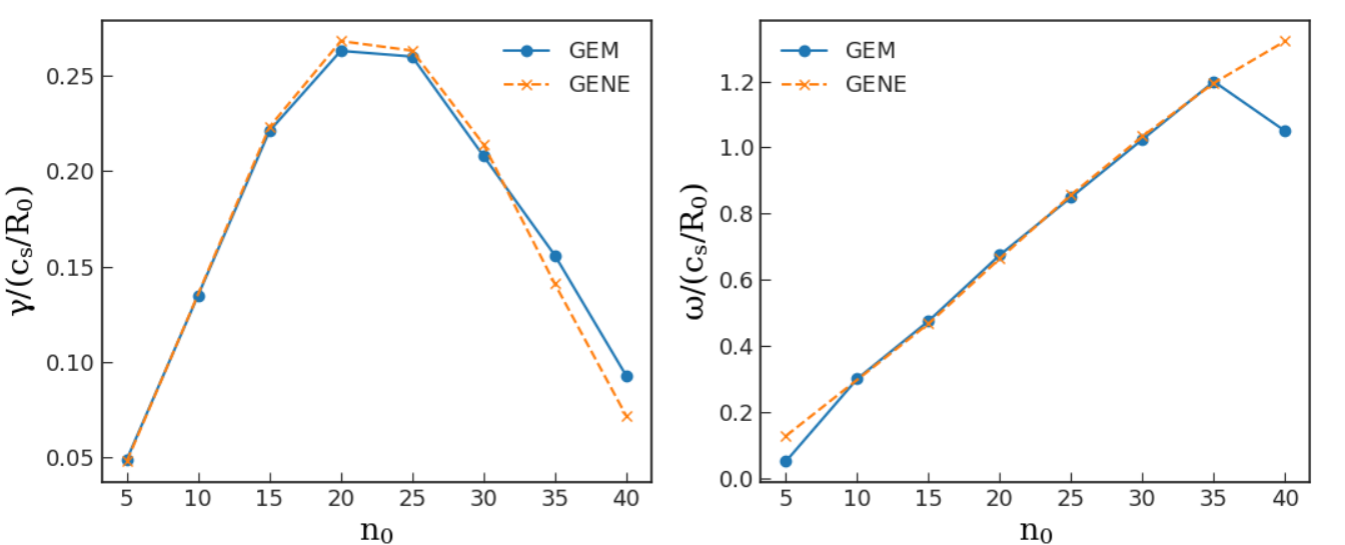
\includegraphics[width=.9\textwidth]{fig1.png}
\caption{hi}
\label{fig1}
\end{figure}
First of all, results of ion temperature gradient (ITG) mode with adiabatic electron response are compared as a baseline
case. As illustrated in figure 1, results obtained by the two codes (GENE and GEM) show a good consistency and conformity 
for both ITG growth rate and frequency, from a scanning over toroidal mode number over $n_0\in$ [5,40]. The GENE results 
correspond to table III and figure 3 in Ref. \cite{gorler}. 



\newpage
\section*{Appendix}\label{app}
We may need the following operator to simplify the coding process.
\begin{equation*}
    \hat{R}\cdot\nabla y = \frac{\partial y}{\partial r}\frac{\partial r}{\partial R} + \frac{r_0}{q_0}\hat{q}\frac{\partial \theta}{\partial R}
\end{equation*}
\begin{equation*}
    \hat{Z}\cdot\nabla y = \frac{\partial y}{\partial r}\frac{\partial r}{\partial Z} + \frac{r_0}{q_0}\hat{q}\frac{\partial \theta}{\partial Z}
\end{equation*}
\begin{equation*}
    \hat{R}\cdot\nabla z = q_0R_0\frac{\partial \theta}{\partial R}
\end{equation*}
\begin{equation*}
    \hat{Z}\cdot\nabla z = q_0R_0\frac{\partial \theta}{\partial Z}
\end{equation*}
\begin{equation*}
    \hat{\zeta}\cdot\nabla y = -\frac{r_0}{q_0R}
\end{equation*}

New variables declared in GEM:\\
omg(nr)---$\omega$, angular frequency of toroidal flow\\
domg(nr)---d$\omega$/dr\\
ut(nr,ntheta)---U, toroidal flow\\
phi1(nr,ntheta)---$\Phi_1$\\
bdgut,bdgbfld,bdgphi1::(nr,ntheta)---${\bf b}\cdot\nabla{\rm U},\ {\bf b}\cdot\nabla{\rm B},\ {\bf b}\cdot\nabla{\rm \Phi_1}$\\
hrdgy(nr,ntheta)---$\hat{R}\cdot\nabla y$\\
hzdgy(nr,ntheta)---$\hat{Z}\cdot\nabla y$\\
hrdgz(nr,ntheta)---$\hat{R}\cdot\nabla z$\\
hzdgz(nr,ntheta)---$\hat{Z}\cdot\nabla z$\\
hztdgy(nr,ntheta)---$\hat{\zeta}\cdot\nabla y$\\
radius2(nr,ntheta)---$R^2$\\
rhoreyp---$\big\langle\rho_R\frac{\partial\phi}{\partial y}\big\rangle$\\
rhozeyp---$\big\langle\rho_Z\frac{\partial\phi}{\partial y}\big\rangle$\\
rhoztexp---$\big\langle\rho_\zeta\frac{\partial\phi}{\partial x}\big\rangle$\\
rhozteyp---$\big\langle\rho_\zeta\frac{\partial\phi}{\partial y}\big\rangle$\\
rhoztezp---$\big\langle\rho_\zeta\frac{\partial\phi}{\partial z}\big\rangle$\\

\newpage
\bibliographystyle{unsrt}
\bibliography{refs}
\end{CJK*}
\end{document}